\section{Research Design}
\label{sec:research-methodology:review}

Research methods are ``a set of organising principles around which empirical data is collection and analysed'' \citep{Easterbrook:2007ws}. \citet{Creswell:2017vn} suggest that strong research design is reflected when the weaknesses of multiple methods complement each other. Using a mixed-methods approach is therefore commonplace in software engineering research, typically due to the human-oriented nature investigating how software engineers work both individually (where methods from psychology may be employed) and together (where methods from sociology may be employed). 

Therefore, studies in software engineering are typically performed as field studies where researchers and developers (or the artefacts they produce) are analysed either directly or indirectly \citep{Singer:2007tu}. The mixed-methods approach combines five classes of field study methods (or empirical strategies/studies) most relevant in empirical software engineering research \citep{Easterbrook:2007ws, Wohlin:2012bu, Juristo:2013vj}: controlled experiments, case studies, survey research, ethnographies, and action research. We chiefly adopt a mixed-methods approach to our work using the \textit{concurrent triangulation} mixed-methods strategy \citep{Jick:1979el} as it best compensates for weaknesses that exist in all research methods, and employs the best strengths of others.



\subsection{Review of Relevant Research Methods}
\label{ssec:research-methodology:review:methods}

Below we review some of the research methods most relevant to our research questions as refined in \cref{sec:research-methodology:research-questions} as presented by \citet{Easterbrook:2007ws}.

\paragraph{Controlled Experiments}
A controlled experiment is an investigation of a clear, testable hypothesis that guides the researcher to decide and precisely measure how at least one independent variable can be manipulated and effect at least one other dependent variable. They determine if the two variables are related and if a cause-effect relationship exists between them. The combination of independent variable values is a \textit{treatment}. It is common to recruit human subjects to perform a task and measure the effect of a randomly assigned treatment on the subjects, though it is not always possible to achieve full randomisation in real-life software engineering contexts, in which case a \textit{quasi-experiment} may be employed where subjects are not randomly assigned to treatments.

While we have defined hypotheses (\rh{1}--\rh{3}), refining them into precise, measurable variables is challenging due to the qualitative nature they present. A well-defined population is also critical and must be easily accessible; the varied range of beginner to expert software engineers with varied understanding of artificial intelligence concepts is required to perform controlled experiments, and thus recruitment may prove challenging. Lastly, the controlled experiment is essentially reductionist by affecting a small amount of variables of interest and controlling all others. This approach is too clinical for the practical outcomes by which our research goals aim for, and is therefore closely tied to the positivist stance.

\paragraph{Case Studies}
Case studies investigate phenomena in their real-life context and are well-suited when the boundary between context and phenomena is unknown \citep{Yin:2017tf}. They offer understanding of how and why certain phenomena occur, thereby investigating ways cause-effect relationships can occur. They can be used to test existing theories (\textit{confirmatory case studies}) by refuting theories in real-world contexts instead of under laboratory conditions or to generate new hypotheses and build theories during the initial investigation of some phenomena (\textit{exploratory case studies}).

Case studies are well-suited where the context of a situation plays a role in the phenomenon being studied, which we specifically relate back to \rh{2} (\ref{rqs:metadata:what-problems-du                                                                e-to-lack-of-metadata} and \ref{rqs:metadata:what-metadata-do-devs-want-and-why}) in exploring whether the context of an application using a \gls{iws} requires the \gls{iws} context-specific or of context-agnostic. They also lend themselves to purposive sampling rather than random sampling, and thus we can selective choose cases that benefit the research goal of \rh{2} and (using our critical theorist stance) select cases that will actively benefit our participant software engineering audience most to draw attention to situations regarded as most problematic.

\paragraph{Survey Research}
Survey research identifies characteristics of a broad population of individuals through direct data collection techniques such as interviews and questionnaires or independent techniques such as data logging. Defining that well-defined population is critical, and selecting a representative sample from it to generalise the data gathered usually assists in answering base-rate questions.

By identifying representative sample of the population, from beginner to experienced developers with varying understanding of \gls{iws} \glspl{api}, we can use survey research to assist in answering our exploratory and base-rate research questions under \rh{1} and \rh{2} (see \cref{ssec:research-methodology:research-questions:knowledge-questions}) in determining the qualitative aspects of how individual developers perceive and work with the existing \glspl{api}, either by directly asking them or by mining third-party discussion websites such as Stack Overflow. However, with direct survey research techniques, low response rates may prove challenging, especially if no inducements can be offered for participation.

\paragraph{Ethnographies}
Ethnographies investigates the understanding of social interaction within community through field observation \citep{Robinson:2007tp}. Resulting ethnographies help understand how software engineering technical communities build practices, communication strategies and perform technical work collaboratively. 

Ethnographies require the researcher to be highly trained in observational and qualitative data analysis, especially if the form of ethnography is participant observation, whereby the researcher is embedded of the technical community for observation. This may require the longevity of the study to be far greater than a couple of weeks, and the researcher must remain part of the project for its duration to develop enough local theories about how the community functions. While it assists in revealing subtle but important aspects of work practices within software teams, this study does not focus on the study of teams, and is therefore not a research method relevant to this project.


\paragraph{Action Research}
Action researchers simultaneously solve real-world problems while studying the experience of solving the problem \citep{Davison:2004wo} by actively seeking to intervene in the situation for the purpose of improving it. A precondition is to engage with a \textit{problem owner} who is willing to collaborate in identifying and solving the problem faced. The problem must be authentic (a problem worth solving) and must have new knowledge outcomes for those involved. It is also characterised as an iterative approach to problem solving, where the knowledge gained from solving the problem has a desirable solution that empowers the problem owner and researcher. 

This research is most associated to our adopted philosophical stance of critical theory. As this project is being conducted under the \gls{a2i2} collaboratively with engaged industry clients, we have identified a need for solving an authentic problem that industry faces. The desired outcome of this project is to facilitate wider change in the usage and development of \glspl{cvs}; thus, engaging action research as a primary method throughout the mixed-methods approach used in this research.

\subsection{Review of Data Collection Techniques for Field Studies}
\label{ssec:research-methodology:review:techniques}

\citeauthor{Singer:2007tu} developed a taxonomy \citep{Singer:2007tu,Lethbridge:2005jv} showcasing data collection techniques in field studies that are used in conjunction with a variety of methods based on the level of interaction between researcher and software engineer, if any. This taxonomy is reproduced in \cref{fig:research-methodology:review:field-techniques}.

\section{Proposed Experiments}
\label{sec:research-methodology:experiments}

This section discusses two proposed experiments that we conduct in this study. For each experiment, we describe an overview of the experiment grounded known methods and techniques (\cref{ssec:research-methodology:review:methods,ssec:research-methodology:review:techniques}), our approach to analysing the data, as well as linking the experiment back to a research hypothesis and question (\cref{sec:introduction:hypohtesis}). A high-level overview of the proposed experiments and the major bodies of work they encompass is presented in \cref{fig:research-methodology:review:activity-diagram}.

\begin{figure}[t!]
  \centering
  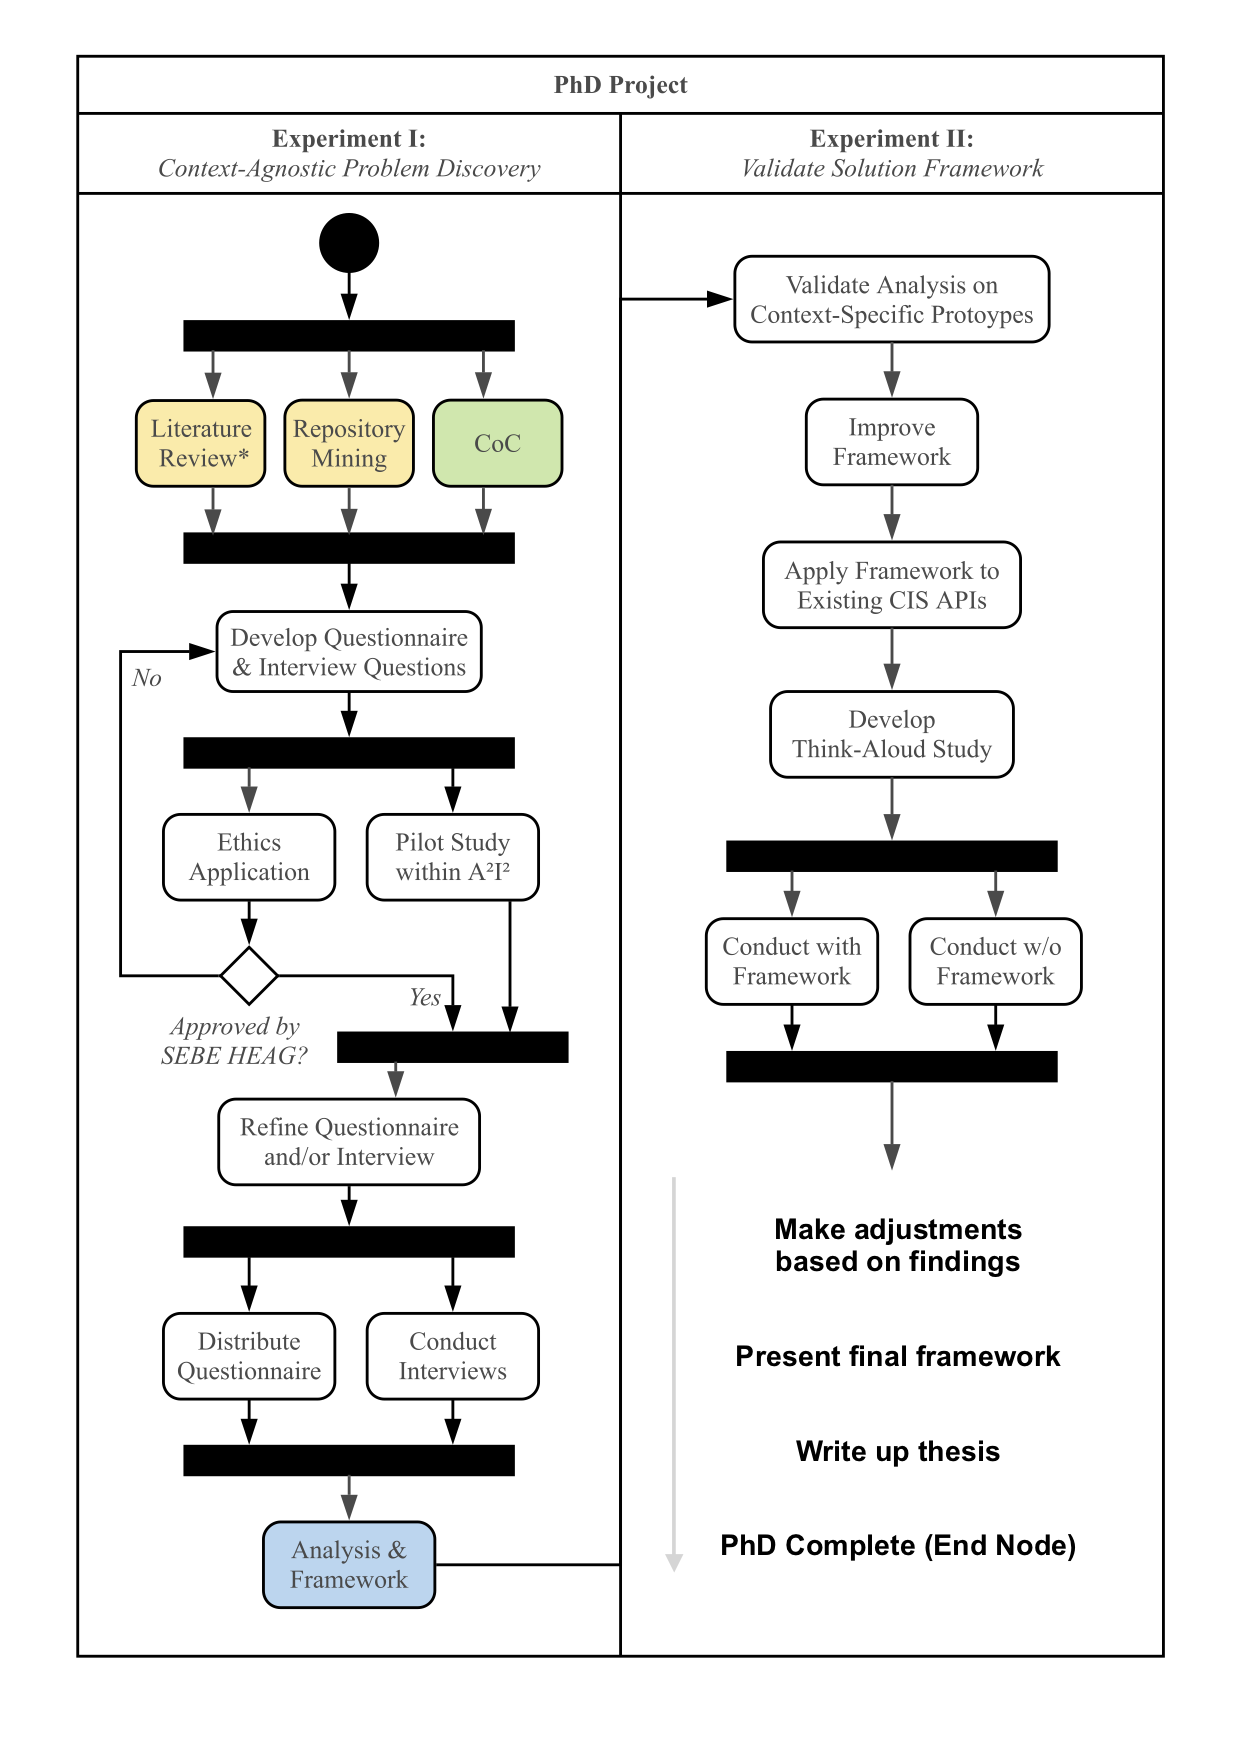
\includegraphics[width=0.9\linewidth]{experiment-activity-diagram}
  \caption[High-level overview of the proposed experiments]{High-level activity diagram of the proposed experiments in this study. Literature review is ongoing.}
  \label{fig:research-methodology:review:activity-diagram}
\end{figure}


\subsection{Experiment I: Develop Initial Framework}
\label{ssec:research-methodology:experiments:1}

Experiment I shapes a context-agnostic approach to understand current usage patterns of \gls{iws} \glspl{api} and the ways by which developers interpret them. Briefly, this experiment is comprised under two phases of field survey research: (i) repository mining developer discussion forums (i.e., analysis of databases and documentation analysis) to understand what developers currently complain about on these forums and where their mismatch in understanding lies; (ii) conducting unstructured interviews and distributing a questionnaire to gather personal opinion based on individual developer's anecdotal remarks.

\subsubsection{Relevance and Motivation}

Experiment I aims to better understand the existing mindsets that developers have when approaching to use \glsplx{cvs}. This work therefore ties in to \rh{1}; by understanding the developer mindset in how they interpret \gls{cvs} \glspl{api}, we are better informed to produce a framework that increases the effectiveness of the documentation of those existing \gls{cvs} providers.

\rh{1} postulates that the software engineering community do not fully understand the `magic' behind \gls{iws} \glspl{api}. As described in \cref{sec:introduction:hypohtesis}, they face a gap in their understanding around the underlying architecture of pre-built, machine learnt \glspl{api} (\ref{rqs:apidoc:how-do-devs-understand-it}). Software developers are not well-supported by the \gls{iws} providers, and therefore do not have a consistent set of common best practices when approaching to use these \glspl{api} (\ref{rqs:apidoc:what-is-in-use}). It is therefore necessary that \gls{iws} providers provide additional information to gap this mismatched understanding (\ref{rqs:apidoc:what-additional-information-needed}). 

\subsubsection{Data Collection \& Analysis}

\paragraph{Phase 1: Repository Mining}
Developers typically congregate in search of discourses on issues they face in online forums, such as Stack Overflow and Quora, as well as writing their experiences in personal blogs such as Medium. The simplest of these platforms is Stack Overflow (a sub-community of the Stack Exchange family of targeted communities) that specifically targets developer issues on using a simple Q\&A interface, where developers can discuss technical aspects and general software development topics. Moreover, Stack Overflow is often acknowledged as \textit{the} `go-to' place for developers to find high-quality code snippets that assist in their problems \citep{Subramanian:2014bg}.

Thus, to begin validating \gls{iws} \gls{api} usage and misunderstanding in a generalised context (i.e., context-agnostic to the project at hand), we propose using repository mining on Stack Overflow to help answer our research questions. Specifically, we select Stack Overflow due to its targeted community of developers\footnote{We also acknowledge that there are other targeted software engineering Stack Exchange communities such as Stack Exchange Software Engineering (\url{https://softwareengineering.stackexchange.com}), though (as of January 2019) this much smaller community consists of only 52,000 questions versus Stack Overflow's 17 million.} and the availability of its publicly available dataset released as `data dumps' on the Stack Exchange Data Explorer\footnoteurl{https://data.stackexchange.com/stackoverflow}{17 January 2017} and Google BigQuery\footnoteurl{https://console.cloud.google.com/marketplace/details/stack-exchange/stack-overflow}{17 January 2017}. Studies conducted have also used Stack Overflow to mine developer discourse \citep{Choi:2015wo,Sinha:2013tt,Novielli:2015vd,Rosen:2016uk,Pal:2012te,Bajaj:2014wg,LinaresVasquez:2014vj,Wang:2013ue,Barua:2012gz,Reboucas:2016tw,Allamanis:2013vb,Tahir:2018ks}.

Due to the enormity of the data produced, we will use qualitative analysis on the questions mined using assistive tools such as NVivo. For this, we will conduct a thematic analysis on the themes of each question mined, the relevance of the question to our research topic, and ensuring strict coding schemes (that reflect our research goals) are adhered to. We refer to \citet{Singer:2007tu} and \citet{Miles:1994ty} on coding and analysing this qualitative data gathered.

\paragraph{Phase 2: Personal Opinion Surveys}
We follow the triangulation approach proposed by \citet{Jick:1979el} to corroborate the qualitative data of developers' discussion of Stack Overflow with secondary survey research, thereby validating what people say on Stack Overflow with what is said and done in real life. \citet{Kitchenham:2007ux} provide an introduction on methods used to conduct personal opinion surveys which we adopt as an initial reference in (i) shaping our survey objectives around our research goals, (ii) designing a cross-sectional survey, (iii) developing and evaluating our two survey instruments (consisting of a structured questionnaire and semi-structured interview), (iv) evaluating our instruments, (v) obtaining the data and (vi) analysing the data.

As is good practice in developing questionnaire instruments to evaluate their reliability and validity \citep{Litwin:1995wt}, we evaluate our instrument design by asking colleagues to critique it via pilot studies within \gls{a2i2}. This assists in identifying any problems with the questionnaire itself and with any issues that may occur with the response rate and follow-up procedures. We follow a similar approach by practicing the interview instrument on colleagues within \gls{a2i2}.

Findings from the pilot study helps inform us for a widely distributed questionnaire and conducting interviews out in the field, where we recruit external software engineers in industry through the industry contacts of \gls{a2i2}. Ethics approval from the Faculty of Science, Engineering and Built Environment Human Ethics Advisory Group (SEBE HEAG) will be required prior to externally conducting this survey research (see \cref{ch:ethics}). The quantitative (survey) and qualitative (interview) analysis allows us to shape the research outcome of \rh{1}---an \gls{api} documentation quality assessment framework---and assists in stabilising our general understanding of how developers use these existing \glspl{api}.

\subsection{Developing the Initial Framework}

Our initial framework is developed using the qualitative and quantitative analyses from the findings of Experiment I. As this is a creative phase in which we are developing a new framework, the exact process by which we develop the initial framework will come to light once more insight is determined. However it is anticipated discussion with other researchers and engineers at \gls{a2i2} about the analyses of the findings (i.e., white-boarding sessions of potential ideas from the findings) will help develop our initial documentation framework. This framework will take the shape of a checklist or table, typical of information systems studies (e.g., \citep{Lau:1999vs}), that indicate what attributes should be best suited for what needs.

\subsection{Experiment II: Validate Initial Framework}
\label{ssec:research-methodology:experiments:2}

Experiment II extends the \textit{generalised} context of Experiment I by evaluating how the findings of Experiment I translates to context-specific applications. We confirm that the generalised findings are (indeed) genuine by conducting action research in combination with an observational study on software engineers. This experiment is also compromised of: (i) development of prototypes using \gls{iws} \glspl{api} of differing contexts; (ii) presenting a solution framework to developers to interpret the improvement of their understanding when using a \gls{iws}.

\subsubsection{Relevance and Motivation}

Experiment II aims to contextualise the findings from Experiment I; that is, if we add \textit{varying contexts} to the applications we write using \gls{iws} \glspl{api}, what is needed to extend the \textit{context-agnostic} framework developed in Experiment I? This work relates back to \rh{2}; adding context-specific metadata to the endpoints of these \glspl{api}, we can highlight what issues exist when such metadata is not present (\ref{rqs:metadata:what-problems-du                                                                e-to-lack-of-metadata}) and what types of metadata developers seek (\ref{rqs:metadata:what-metadata-do-devs-want-and-why}).

Moreover, the implication of the first two hypotheses suggest that applying an \gls{api} documentation and metadata quality assessment framework may have an effect on other aspects within the software engineering process (\rh{3}). Thus, this experiment also confirms if our framework makes an improvement to software quality, developer productivity and/or developer informativeness (\ref{rqs:implications:do-metrics-improve} and \ref{rqs:implications:aspects}).

\subsubsection{Data Collection \& Analysis}

To confirm findings of the method within \rh{1} is genuine, we shift from reviewing the documentation from a general stance to a specialised (context-specific) stance in the use of these \glspl{api}.

This is firstly achieved by using existing \gls{iws} \glspl{api} to develop basic `prototypes', each having differing contexts. The number of prototypes to develop and the use cases they have will be informed by the results of Experiment I, and therefore cannot yet be described at this stage. Our action research in developing the prototypes will help inform any potential gaps that exist in the findings of \rh{1}, especially with regards to context-specifity, and therefore improves the metadata component of our framework (as per the outcome of \rh{2}). 

This outcome will also help us design the next stage of the experiment, consisting of a comparative controlled study \citep{Seaman:2007wa} to capture firsthand behaviours and interactions toward how software engineers approach using a \gls{iws} with and without our framework applied. We will provide improved documentation and metadata responses of a set of popular \glspl{cvs} that is documented with the additional metadata and whose information is organised using our framework. 

We then recruit 20 developers of varying experience (from beginner programmer to principal engineer) to complete five tasks under an observational, comparative controlled study, 10 of which will (a) develop with the \textit{new} framework, and the other 10 will (b) develop with the \textit{as-is/existing} documentation. From this, we compare if the framework makes improvements by capturing metrics and recording the observational sessions for qualitative analysis. We use visual modelling to analyse the qualitative data using matrices \citep{Dey:2003ty}, maps and networks \citep{Miles:1994ty} as these help illustrate any causal, temporal or contextual relationships that may exist to map out the developer's mindset and difference in approaching the two sets of designs of the same tasks.

%To validate the findings of developer opinion in the surveys and interviews of \rh{1} are indeed genuine, this helps ensure that there is nothing missing by adding in further context to such opinions.

%\subsection{Primary Contributions arising from Experiments I and II}
%\label{ssec:research-methodology:experiments:contribution}
%
%Ultimately, we seek to understand the conceptual understanding of software engineers who operationalise stochastic and probabilistic systems, and furthermore understand knowledge representation with these systems' \gls{api} documentation. Our motivation is to provide insight into current practices and compare the best practices with actual practise. We strive for this to  provide developers with a guiding framework on how to best operationalise these systems via the form of some checklist or tool they can use to ensure optimal software quality.
%
%It is anticipated that the findings from this study in the \glspl{cvs} space will be generalisable to other areas, such as time-series information, natural language processing and others.
